% Provenance (never printed): old seconde/premiere S material on the water
% cycle on land (the drainage basin, river discharge, floods and their
% management); see sources/book2/PROVENANCE.md. The Varden basin is computed
% in figdata/grade-10/varden_basin.py from figdata/shared/region.py; the
% Potomac record in figdata/grade-10/flood_frequency.py.
\chapter{Stroomgebieden, rivieren en hoogwater}\label{ch:g10:drainage-basins}

Een rivier kan twee dagen nadat de regen is opgehouden stijgen, bij een stad
waar helemaal geen regen is gevallen. Het water dat haar straten overstroomt,
viel eerder, op heuvels ver stroomopwaarts; het liep van hun hellingen naar
beken, en de beken kwamen samen in de rivier die het, allemaal tegelijk, naar de
stad bracht. Om een overstroming te begrijpen, moet je verder kijken dan de
rivier, naar het hele gebied dat haar voedt, en het water daardoorheen volgen.
Dit hoofdstuk definieert dat gebied, het \omterm{def:g10:drainage-basins:drainage-basin}{stroomgebied}; meet wat een rivier
vervoert, haar \omterm{def:g10:drainage-basins:discharge}{afvoer}; volgt een hoogwater terwijl het een punt van de rivier
passeert; en laat zien hoe een lange reeks hoogwaters vertelt hoe vaak een
bepaald hoogwater terugkomt.

\begin{omfigure}
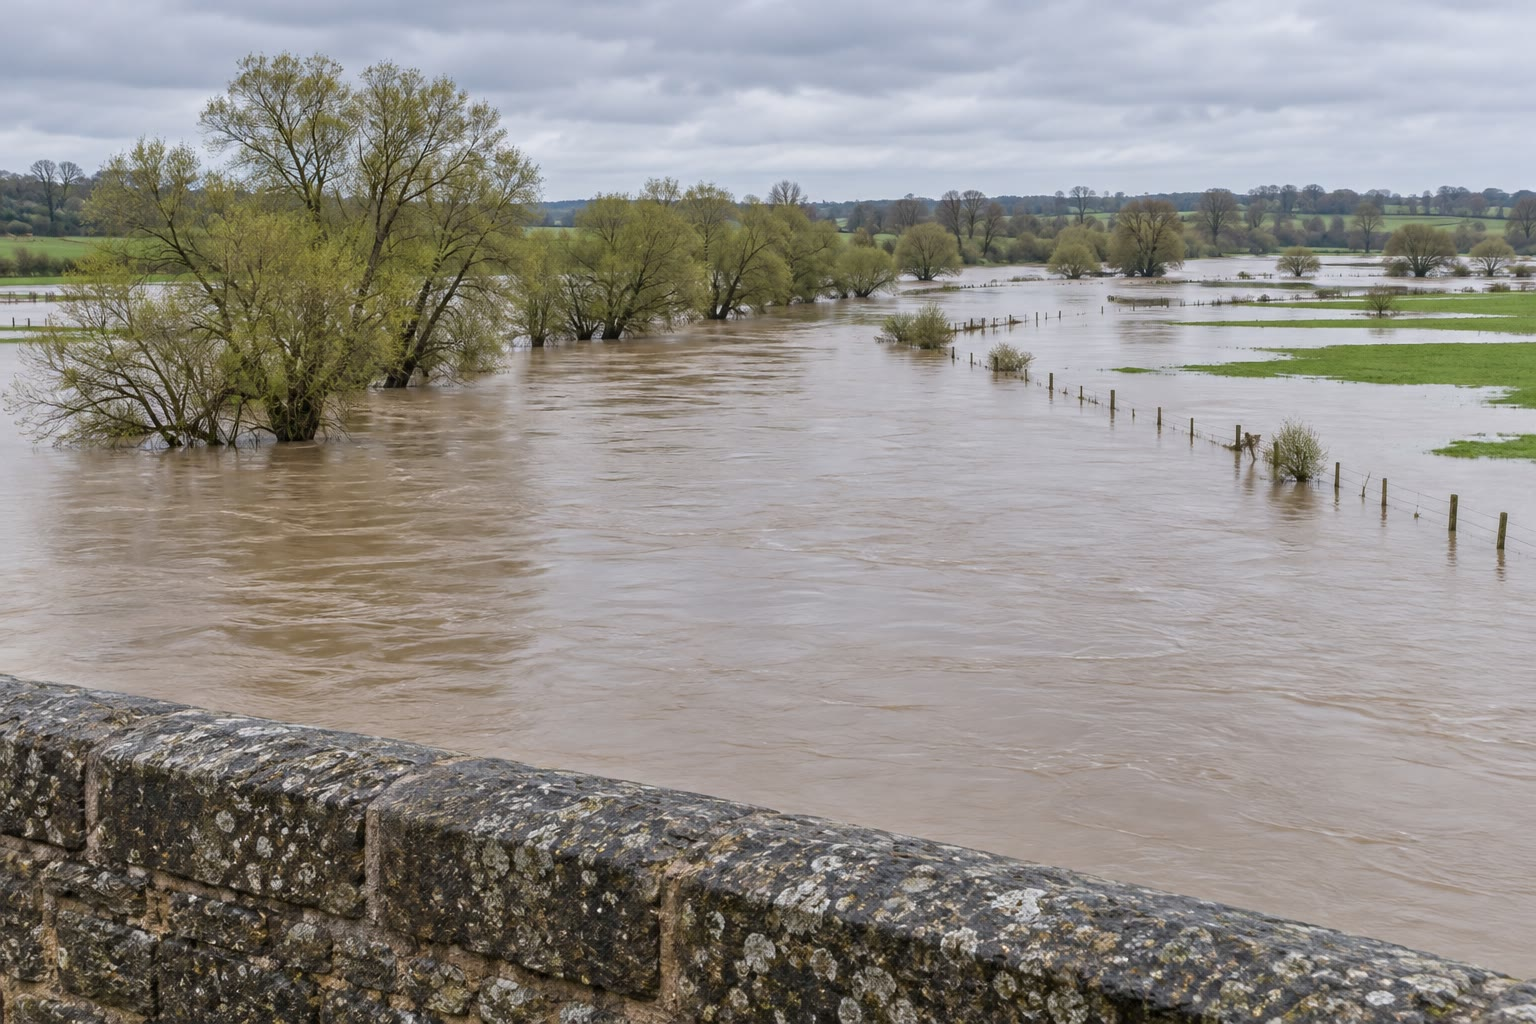
\includegraphics[width=0.8\linewidth]{images/book2/ai/g10-river-flood-meadows.jpg}

{\small Een rivier die buiten haar oevers is getreden, gezien vanaf een stenen
brug: het bruine, met slib beladen water heeft zijn bedding verlaten en bedekt
de weiden van de overstromingsvlakte, tot aan de hekken en de bomen die
normaal langs de oevers staan.}
\end{omfigure}

\begin{recall}
Regen die de grond bereikt, zakt erin weg, stroomt over het oppervlak af of
verdampt; de waterkringloop brengt hem terug naar zee (de natuurkundeboeken).
Water zakt weg in doorlatende gesteenten en vult ze onder de grondwaterspiegel,
waardoor watervoerende lagen ontstaan die bronnen en rivieren voeden (Boek 1,
jaar 6). Een rivier slingert in meanders over haar vlakke overstromingsvlakte,
die ze bij hoogwater bedekt (Boek 1, jaar 5). Hoogtelijnen verbinden punten van
gelijke hoogte; de Varden Hills zijn het gebied dat op de kaarten van deze reeks
is getekend (Boek 1, jaren 2 en 9).
\end{recall}

\begin{safety}
Overstromingswater is veel gevaarlijker dan het lijkt. Ongeveer \qty{15}{cm}
snelstromend water kan een volwassene omverduwen, en ongeveer \qty{30}{cm} kan
een auto meevoeren; de weg eronder kan zijn ingestort. Loop of rijd nooit door
overstromingswater: keer om en neem een andere weg.
% ledger: nws:flood-water
\end{safety}

\section{Het stroomgebied}

Elke regendruppel die niet verdampt of diep wegzakt, stroomt bergafwaarts. Hij
volgt de steilste helling van de grond, komt in een geultje terecht, dan in een
beek, en de beken komen samen in rivieren. Al het land waarvan het water in
dezelfde rivier eindigt, vormt één geheel.

\begin{definition}[Stroomgebied; waterscheiding]\label{def:g10:drainage-basins:drainage-basin}
Het \emph{stroomgebied}\index{stroomgebied} van een punt van een rivier is het
hele landoppervlak waarvan het afstromende water stroomopwaarts van dat punt
naar de rivier stroomt en dat punt passeert. De
\emph{waterscheiding}\index{waterscheiding} is de lijn die twee aangrenzende
stroomgebieden scheidt: ze volgt de kammen van het land, en de regen die aan
weerszijden ervan valt, stroomt naar verschillende rivieren.
\end{definition}

Een \omterm{def:g10:drainage-basins:drainage-basin}{stroomgebied} wordt altijd gedefinieerd voor een punt van de rivier, zijn
\emph{uitstroompunt}: het \omterm{def:g10:drainage-basins:drainage-basin}{stroomgebied} van een rivier waar ze de zee bereikt, is
het grootste, en elk punt stroomopwaarts heeft een kleiner \omterm{def:g10:drainage-basins:drainage-basin}{stroomgebied} daarbinnen.
Twee druppels die een meter uit elkaar vallen, aan weerszijden van een
\omterm{def:g10:drainage-basins:drainage-basin}{waterscheiding}, kunnen in verschillende rivieren en zelfs in verschillende
oceanen terechtkomen.

\subsection*{Het stroomgebied van de Varden}

Een computer vindt een \omterm{def:g10:drainage-basins:drainage-basin}{stroomgebied} in een paar stappen uit een hoogtekaart. De
kaart wordt in kleine vierkantjes verdeeld, hier met zijden van \qty{50}{m}.
Voor elk vierkantje bekijkt de computer zijn acht buren en stuurt hij het water
naar de buur die via de steilste helling naar beneden bereikt wordt. (Waar een
kleine kom geen lagere buur heeft, wordt die eerst opgevuld tot het niveau
waarop ze zou overlopen, zoals een plas dat doet.) Wie deze stappen van
vierkantje tot vierkantje volgt, vindt de weg van een druppel vanaf elke plaats
op de kaart. De vierkantjes waarvan de druppels de rivier bereiken, vormen het
\omterm{def:g10:drainage-basins:drainage-basin}{stroomgebied}.

\begin{omfigure}
\begin{tikzpicture}
\begin{axis}[axis equal image, xmin=0, xmax=10, ymin=0, ymax=8, width=0.86\linewidth,
  tick label style={font=\scriptsize}, xlabel={oost (km)}, ylabel={noord (km)},
  label style={font=\small}, enlargelimits=false]
\addplot[fill=omDef!14, draw=none, even odd rule] table {figdata/out/grade-10-varden_basin-fill.dat};
\addplot[contour, line width=0.25pt, opacity=0.7] table {figdata/out/shared-region-contours.dat};
\addplot[index contour, opacity=0.8] table {figdata/out/shared-region-index-contours.dat};
\addplot[river, line width=1.6pt] table {figdata/out/shared-region-river.dat};
\addplot[omThm, line width=1.4pt, dashed] table {figdata/out/grade-10-varden_basin-divide.dat};
\addplot[omWxRain, line width=0.9pt, -{Stealth[length=5pt]}] table {figdata/out/grade-10-varden_basin-path1.dat};
\addplot[omWxRain, line width=0.9pt, -{Stealth[length=5pt]}] table {figdata/out/grade-10-varden_basin-path2.dat};
\addplot[omWxRain, line width=0.9pt, -{Stealth[length=5pt]}] table {figdata/out/grade-10-varden_basin-path3.dat};
\addplot[omWxRain, line width=0.9pt, -{Stealth[length=5pt]}] table {figdata/out/grade-10-varden_basin-path4.dat};
\fill[omWxRain] (axis cs:2,7.4) circle (2.2pt);
\fill[omWxRain] (axis cs:4,1.8) circle (2.2pt);
\fill[omWxRain] (axis cs:8.6,6.6) circle (2.2pt);
\fill[omWxRain] (axis cs:2.5,0.7) circle (2.2pt);
\node[font=\footnotesize, fill=white, fill opacity=0.85, text opacity=1, inner sep=1.5pt, text=omThm] at (axis cs:6.0,6.75) {waterscheiding};
\node[font=\footnotesize, fill=white, fill opacity=0.85, text opacity=1, inner sep=1.5pt, text=omThm] at (axis cs:3.5,1.1) {waterscheiding};
\node[font=\footnotesize, fill=white, fill opacity=0.85, text opacity=1, inner sep=1.5pt, align=center] at (axis cs:5.3,7.55) {buiten het stroomgebied:\\water stroomt naar het noorden weg};
\node[font=\footnotesize, fill=white, fill opacity=0.85, text opacity=1, inner sep=1.5pt, align=right, anchor=east] at (axis cs:9.85,3.35) {uitstroompunt};
\draw[-{Stealth[length=6pt]}, line width=1pt, omRiver] (axis cs:9.3,3.7) -- (axis cs:9.95,4.15);
\node[font=\footnotesize, fill=white, fill opacity=0.85, text opacity=1, inner sep=1.5pt] at (axis cs:1.1,4.75) {rivier};
\end{axis}
\end{tikzpicture}

{\small Het \omterm{def:g10:drainage-basins:drainage-basin}{stroomgebied} van de Varden op de kaart van de Varden Hills
(gearceerd), berekend door het water van elk vierkantje van \qty{50}{m} langs de
steilste helling naar beneden te sturen; hoogtelijnen om de \qty{50}{m}. De
stippellijnen zijn de \omterm{def:g10:drainage-basins:drainage-basin}{waterscheidingen}; de blauwe lijnen zijn de wegen van vier
regendruppels (stippen). Twee bereiken de rivier en stromen naar het oosten
naar het uitstroompunt, waar de rivier de kaart verlaat; de twee andere, voorbij
de \omterm{def:g10:drainage-basins:drainage-basin}{waterscheidingen}, verlaten de kaart in de richting van andere rivieren.}
\end{omfigure}

Het \omterm{def:g10:drainage-basins:drainage-basin}{stroomgebied} beslaat \qty{66}{km^2} van de \qty{80}{km^2} van de kaart,
ongeveer vier vijfde ervan. In het noorden volgt de \omterm{def:g10:drainage-basins:drainage-basin}{waterscheiding} de kammen van
de heuvels en loopt ze over hun toppen; daarachter helt het land van de rivier af
en stroomt het water naar een ander dal. In de zuidwesthoek watert ook een klein
gebied van de kaart af. De rivier zelf komt de kaart vanuit het westen binnen,
zodat haar volledige \omterm{def:g10:drainage-basins:drainage-basin}{stroomgebied} groter is: het omvat ook het land
stroomopwaarts, voorbij de rand van de kaart.
% values computed in figdata/grade-10/varden_basin.py (basin_km2 66.19, map_km2 80)

\subsection*{De grootste rivieren}

Rivieren worden vergeleken naar de oppervlakte van hun \omterm{def:g10:drainage-basins:drainage-basin}{stroomgebied} en naar het
water dat ze vervoeren. De verreweg grootste rivier ter wereld is de Amazone. De
Mississippi, de grootste rivier van de Verenigde Staten, ontwatert ongeveer
\num{1150000} vierkante mijl, ongeveer 2.98 miljoen \unit{km^2}, van de Verenigde
Staten en Canada.
% ledger: kammerer:mississippi

\section{Afvoer}

\begin{definition}[Afvoer]\label{def:g10:drainage-basins:discharge}
De \emph{afvoer}\index{afvoer} van een rivier op een punt is het volume water dat
in één seconde door een dwarsdoorsnede van de rivier stroomt. Ze wordt gemeten
in kubieke meter per seconde, \unit{m^3/s}.
\end{definition}

Een \omterm{def:g10:drainage-basins:discharge}{afvoer} van \qty{1}{m^3/s} is duizend liter per seconde, of
\qty{86400}{m^3} per dag. Het water stroomt het snelst dicht bij het oppervlak
in het midden van de bedding en het traagst langs de bodem en de oevers, waar het
ertegen schuurt; de \emph{gemiddelde stroomsnelheid} is de snelheid, gemiddeld
over de hele dwarsdoorsnede.

\begin{proposition}[Afvoer, stroomsnelheid en dwarsdoorsnede]\label{prop:g10:drainage-basins:discharge}
De \omterm{def:g10:drainage-basins:discharge}{afvoer} $Q$ van een rivier is het product van de gemiddelde snelheid $v$ van
het water en de oppervlakte $A$ van de natte dwarsdoorsnede:
\[
Q = v\,A.
\]
\end{proposition}

\begin{proof}
In een tijd $t$ is het water dat de doorsnede passeert een afstand $v\,t$ vooruit
gegaan: het vult een plak van de rivier met doorsnede $A$ en lengte $v\,t$, met
volume $A\,v\,t$. Dit volume delen door de tijd $t$ geeft het volume per
seconde, $Q = v\,A$.
\end{proof}

Een rivier met een dwarsdoorsnede van \qty{50}{m^2} die met een gemiddelde
snelheid van \qty{1.2}{m/s} stroomt, voert $1.2 \times 50 = \qty{60}{m^3/s}$ af.
Bij hoogwater nemen beide factoren toe: het water wordt dieper en breder, zodat
de dwarsdoorsnede groeit, en het stroomt sneller.

\subsection*{Een afvoer meten}

Omdat de snelheid over de breedte van de rivier verandert, wordt ze op
verscheidene punten gemeten. De rivier wordt in verticale stroken verdeeld; in
elke strook worden de diepte en de snelheid gemeten, en de \omterm{def:g10:drainage-basins:discharge}{afvoeren} van de
stroken worden opgeteld.

\begin{method}[De snelheid-oppervlaktemethode]\label{met:g10:drainage-basins:velocity-area}
\begin{enumerate}
  \item Span een meetlint over de rivier en kies verticalen op regelmatige
        afstanden $w$ langs het lint.
  \item Meet bij elke verticaal de diepte $d$ en, met een stroomsnelheidsmeter,
        de gemiddelde snelheid $v$ van het water over die diepte.
  \item Elke verticaal staat voor een strook met breedte $w$ en oppervlakte
        $w\,d$; de \omterm{def:g10:drainage-basins:discharge}{afvoer} ervan is $v\,w\,d$.
  \item Tel de \omterm{def:g10:drainage-basins:discharge}{afvoeren} van alle stroken op: $Q = \sum v\,w\,d$.
        De dwarsdoorsnede is $A = \sum w\,d$ en de gemiddelde snelheid $Q/A$.
\end{enumerate}
\end{method}

\begin{omfigure}
\begin{tikzpicture}[x=0.9cm, y=1.6cm, font=\footnotesize]
  % water
  \fill[omSea] (0,0) -- (1,-0.4) -- (2,-0.75) -- (3,-1.0) -- (4,-1.25) -- (5,-1.4) -- (6,-1.3)
     -- (7,-1.1) -- (8,-0.8) -- (9,-0.5) -- (10,-0.2) -- (10.5,0) -- cycle;
  \fill[omDef!22] (4,0) -- (4,-1.25) -- (5,-1.4) -- (6,-1.3) -- (6,0) -- cycle;
  % bed
  \draw[line width=0.9pt, brown!60!black] (-0.6,0.35) -- (0,0) -- (1,-0.4) -- (2,-0.75) -- (3,-1.0) -- (4,-1.25)
     -- (5,-1.4) -- (6,-1.3) -- (7,-1.1) -- (8,-0.8) -- (9,-0.5) -- (10,-0.2) -- (10.5,0) -- (11.1,0.35);
  \draw[omDef!70!black, line width=0.5pt] (0,0) -- (10.5,0);
  % verticals
  \foreach \x/\d/\v/\dx in {1/0.4/0.3/0.3, 3/1.0/0.6/0, 5/1.4/0.8/0, 7/1.1/0.7/0, 9/0.5/0.4/-0.25} {
    \draw[black!70, dashed] (\x,0) -- (\x,-\d);
    \node[anchor=south, font=\scriptsize] at (\x,0.02) {\qty{\v}{m/s}};
    \node[font=\scriptsize, fill=white, inner sep=0.8pt] at (\x+\dx,-0.5*\d) {\qty{\d}{m}};
  }
  \draw[{Stealth}-{Stealth}] (4,0.42) -- node[above, font=\scriptsize] {één strook: $w = \qty{2}{m}$} (6,0.42);
  \node[anchor=west, align=left] at (11.2,-0.15) {water-\\oppervlak};
  \node[anchor=west, align=left] at (11.2,-0.9) {bodem};
  \draw[black!50] (11.15,-0.9) -- (8.5,-0.68);
  \node[anchor=north] at (5.25,-1.75) {gemiddelde snelheden gemeten bij de verticalen (boven het water) en diepten (in het water)};
\end{tikzpicture}

{\small Een \omterm{def:g10:drainage-basins:discharge}{afvoer} meten (schematisch; verticale schaal overdreven). Vijf
verticalen, \qty{2}{m} uit elkaar, verdelen een beek van ongeveer \qty{10}{m}
breed in stroken; de gearceerde strook is die van de middelste verticaal.}
\end{omfigure}

\begin{example}[Een afvoermeting]\label{ex:g10:drainage-basins:gauging}
In de beek van de figuur hebben de vijf stroken, elk \qty{2}{m} breed,
oppervlakten van $2 \times 0.4 = 0.8$, $2.0$, $2.8$, $2.2$ en \qty{1.0}{m^2}: de
dwarsdoorsnede is \qty{8.8}{m^2}. Hun \omterm{def:g10:drainage-basins:discharge}{afvoeren} zijn $0.3 \times 0.8 =
0.24$, $0.6 \times 2.0 = 1.20$, $0.8 \times 2.8 = 2.24$, $0.7 \times 2.2 =
1.54$ en $0.4 \times 1.0 = \qty{0.40}{m^3/s}$, dus de beek voert
$Q \approx \qty{5.6}{m^3/s}$ af. De gemiddelde snelheid is $5.62/8.8 \approx
\qty{0.64}{m/s}$, minder dan de \qty{0.8}{m/s} in het midden van de beek.
\end{example}

\begin{omfigure}
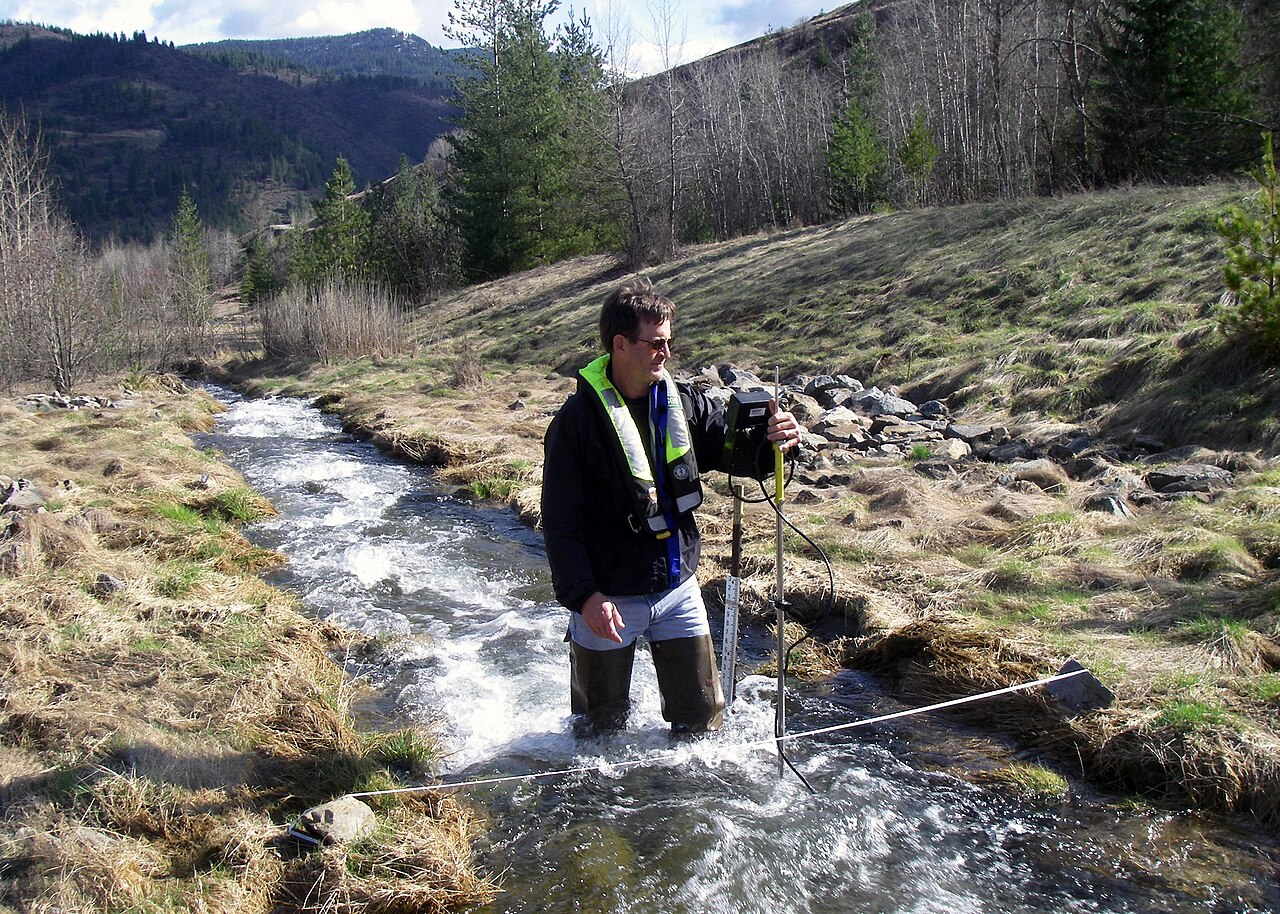
\includegraphics[height=4.6cm]{images/book2/g10-usgs-hydrologist-streamflow.jpg}\hspace{0.3cm}%
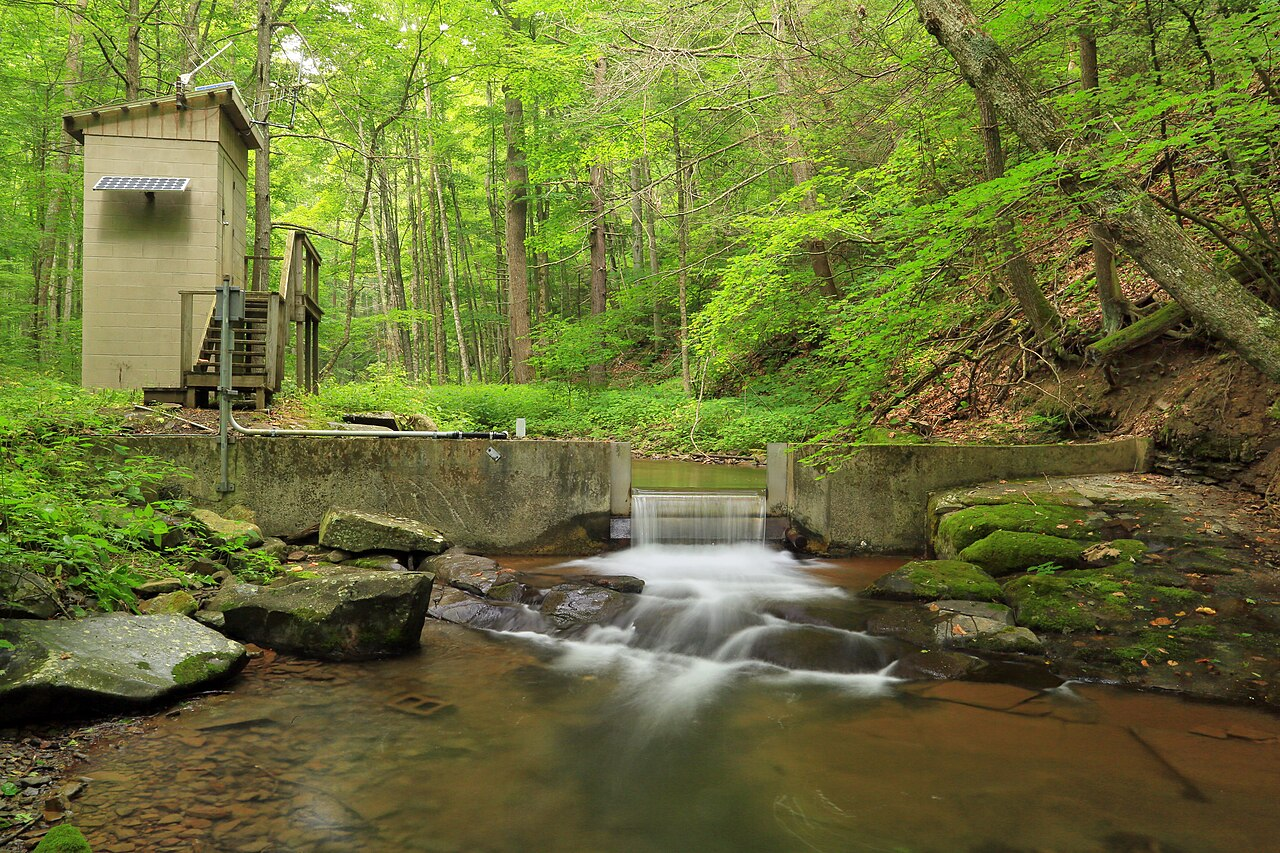
\includegraphics[height=4.6cm]{images/book2/g10-usgs-streamgage.jpg}

{\small Links: een hydroloog meet de \omterm{def:g10:drainage-basins:discharge}{afvoer} van een bergbeek met de
snelheid-oppervlaktemethode; het meetlint dat over de beek is gespannen, markeert
de verticalen, en de stang draagt een stroomsnelheidsmeter. Rechts: een
meetstation aan een bosbeek; het hutje bevat de instrumenten die het waterpeil
achter de kleine stuw registreren. Foto's: U.S. Geological Survey
(publiek domein).}
\end{omfigure}

Een afvoermeting kost tijd en kan niet continu worden uitgevoerd. Een meetstation
registreert in plaats daarvan het waterpeil, zonder onderbreking. Een paar
afvoermetingen bij verschillende peilen geven een kromme die het peil aan de
\omterm{def:g10:drainage-basins:discharge}{afvoer} koppelt, en het station zet elk peil dat het registreert om in een \omterm{def:g10:drainage-basins:discharge}{afvoer}.

Grote rivieren voeren enorme hoeveelheden water af. Van 1972 tot 2003 leverde de
Amazone gemiddeld ongeveer \qty{206000}{m^3/s} aan de Atlantische Oceaan, op
ongeveer \qty{6}{\percent} nauwkeurig: ongeveer \qty{17}{\percent} van al het
zoete water dat de rivieren van de wereld naar zee brengen. De Mississippi
brengt gemiddeld \num{593000} kubieke voet per seconde, ongeveer
\qty{16800}{m^3/s}, naar de Golf van Mexico: de Amazone voert zo'n twaalf keer
meer af.
% ledger: callede:amazon, kammerer:mississippi

\section{De hydrograaf}

\begin{definition}[Hydrograaf; basisafvoer; vertragingstijd]\label{def:g10:drainage-basins:hydrograph}
Een \emph{hydrograaf}\index{hydrograaf} is de grafiek van de \omterm{def:g10:drainage-basins:discharge}{afvoer} van een
rivier op één punt tegen de tijd. De \emph{basisafvoer}\index{basisafvoer} is
het deel van de \omterm{def:g10:drainage-basins:discharge}{afvoer} dat door grondwater wordt gevoed, en dat de rivier tussen
regenbuien laat stromen. De \emph{vertragingstijd}\index{vertragingstijd} van een
hoogwater is de tijd tussen de piek van de neerslag op het \omterm{def:g10:drainage-basins:drainage-basin}{stroomgebied} en de
piek van de \omterm{def:g10:drainage-basins:discharge}{afvoer}.
\end{definition}

\begin{omfigure}
\begin{tikzpicture}[x=1cm, y=1cm, font=\footnotesize]
  \draw[-{Stealth}] (0,0) -- (10.2,0) node[below left] {tijd};
  \draw[-{Stealth}] (0,0) -- (0,5.9) node[above right] {afvoer};
  % rain bars hanging from the top
  \draw[black!50] (0,5.4) -- (10,5.4);
  \foreach \x/\h in {1.0/0.15, 1.3/0.35, 1.6/0.55, 1.9/0.4, 2.2/0.2} {
    \fill[omWxRain!70] (\x,5.4) rectangle ++(0.28,-\h);
  }
  \node[anchor=south west] at (2.6,5.4) {neerslag op het stroomgebied};
  % baseflow and hydrograph
  \fill[omSea] (0,0.7) -- (2.0,0.7) .. controls (2.8,0.8) and (3.3,3.3) .. (4.0,3.6)
    .. controls (4.6,3.6) and (5.1,2.1) .. (6.0,1.55) .. controls (7.0,1.0) and (8.0,0.85) .. (10,0.8)
    -- (10,0) -- (0,0) -- cycle;
  \fill[omLithAlluv] (0,0) -- (0,0.7) -- (2.0,0.7) .. controls (3.5,0.68) and (5.5,0.75) .. (6.6,0.95)
    .. controls (8,1.0) and (9,0.85) .. (10,0.8) -- (10,0) -- cycle;
  \draw[omDef, line width=1.2pt] (0,0.7) -- (2.0,0.7) .. controls (2.8,0.8) and (3.3,3.3) .. (4.0,3.6)
    .. controls (4.6,3.6) and (5.1,2.1) .. (6.0,1.55) .. controls (7.0,1.0) and (8.0,0.85) .. (10,0.8);
  \draw[black!60, dashed] (2.0,0.7) .. controls (3.5,0.68) and (5.5,0.75) .. (6.6,0.95);
  % lag time
  \draw[black!60, densely dotted] (1.74,4.85) -- (1.74,4.3);
  \draw[black!60, densely dotted] (3.98,3.65) -- (3.98,4.3);
  \draw[{Stealth}-{Stealth}] (1.74,4.3) -- node[above] {vertragingstijd} (3.98,4.3);
  % labels
  \node[anchor=west] at (4.2,3.75) {piek};
  \node[anchor=east, align=right] at (2.9,2.2) {stijgende\\tak};
  \node[anchor=west, align=left] at (5.4,2.3) {dalende tak};
  \node[align=center] at (4.5,1.25) {afstroming};
  \node at (8.2,0.4) {basisafvoer};
\end{tikzpicture}

{\small De \omterm{def:g10:drainage-basins:hydrograph}{hydrograaf} van een hoogwater (schematisch). Na de regen stijgt de
\omterm{def:g10:drainage-basins:discharge}{afvoer} tot een piek en daalt ze langzamer weer; de oppervlakte onder de kromme is
het volume water. De \omterm{def:g10:drainage-basins:hydrograph}{basisafvoer}, gevoed door grondwater, verandert weinig; de
rest is het afstromende water dat de regen snel naar de rivier stuurde.}
\end{omfigure}

Het water van een bui bereikt de rivier op verschillende tijdstippen. Regen die
dicht bij de bedding valt, komt binnen minuten of uren aan; regen die ver
stroomopwaarts valt, doet er veel langer over, omdat hij langs de hellingen en
langs de rivier naar beneden moet stromen. De \omterm{def:g10:drainage-basins:discharge}{afvoer} stijgt daarom steil, op de
\emph{stijgende tak}, terwijl het water van de nabije hellingen aankomt, bereikt
een piek wanneer het meeste water tegelijk aankomt, en daalt langzamer, op de
\emph{dalende tak}, terwijl het laatste water uit de verre hoeken van het
\omterm{def:g10:drainage-basins:drainage-basin}{stroomgebied} en uit de bodem wegloopt. Hoe groter het \omterm{def:g10:drainage-basins:drainage-basin}{stroomgebied}, hoe langer de
\omterm{def:g10:drainage-basins:hydrograph}{vertragingstijd}: uren voor een kleine beek, dagen voor een grote rivier.

Sommige \omterm{def:g10:drainage-basins:drainage-basin}{stroomgebieden} geven \emph{plotselinge} hoogwaters, met een hoge,
abrupte piek en een korte \omterm{def:g10:drainage-basins:hydrograph}{vertragingstijd}; andere geven trage, vlakke
hoogwaters. Dezelfde regen geeft een plotselinger hoogwater wanneer:
\begin{itemize}
  \item het \omterm{def:g10:drainage-basins:drainage-basin}{stroomgebied} klein en steil is, zodat het water een korte, snelle
        weg te gaan heeft;
  \item de grond weinig water laat wegzakken: kale rots, klei, grond die al
        doorweekt is, bevroren grond, en vooral de daken, wegen en parkeerterreinen
        van een stad, die bijna alle regen rechtstreeks naar riolen en beken
        sturen;
  \item het \omterm{def:g10:drainage-basins:drainage-basin}{stroomgebied} een dicht netwerk van beken en riolen heeft, dat het
        water snel verzamelt.
\end{itemize}
Bossen, diepe doorlatende bodems en brede overstromingsvlakten doen het
omgekeerde: ze houden het water vast en geven het langzaam af, wat de piek
verlaagt en vertraagt.

\subsection*{Een echt hoogwater}

De Potomac ontwatert stroomopwaarts van een meetstation bij Washington, in het
oosten van de Verenigde Staten, een \omterm{def:g10:drainage-basins:drainage-basin}{stroomgebied} van \num{11560} vierkante mijl,
ongeveer \qty{29900}{km^2}. In januari 1996 registreerde het station de
\omterm{def:g10:drainage-basins:hydrograph}{hydrograaf} hieronder.
% ledger: data:b2-usgs-potomac

\begin{omfigure}
\begin{tikzpicture}
\begin{axis}[omrecord, width=0.86\linewidth, height=6cm, xmin=0, xmax=55, ymin=0, ymax=10000,
  xtick={0,10,20,30,40,50}, xticklabels={5 jan, 15 jan, 25 jan, 4 feb, 14 feb, 24 feb},
  ylabel={afvoer (\unit{m^3/s})}, xlabel={1996},
  tick label style={font=\small}, label style={font=\small},
  scaled y ticks=false, yticklabel style={/pgf/number format/fixed}]
\addplot[omDef, line width=1.1pt, mark=*, mark size=1.1pt] table[x=day, y=q] {figdata/out/grade-10-flood_frequency-hydrograph.dat};
\node[anchor=west, font=\footnotesize] at (axis cs:17,9231) {\qty{9231}{m^3/s} op 21 januari};
\draw[black!60, dashed] (axis cs:5,334) -- (axis cs:13,334);
\node[anchor=south, font=\footnotesize] at (axis cs:9,1000) {ongeveer \qty{330}{m^3/s}};
\draw[black!60] (axis cs:9,1000) -- (axis cs:9,390);
\end{axis}
\end{tikzpicture}

{\small Daggemiddelde \omterm{def:g10:drainage-basins:discharge}{afvoer} van de Potomac bij Washington van 5 januari tot
29 februari 1996: het hoogwater steeg van \qty{362}{m^3/s} op 18 januari
tot meer dan \qty{9000}{m^3/s} drie dagen later, en zakte daarna in de weken
erna weer terug, met een kleinere tweede stijging eind januari.
Gegevens: U.S. Geological Survey, station 01646500.}
\end{omfigure}
% values computed in figdata/grade-10/flood_frequency.py (hydro_peak_m3s 9231, hydro_before_mean 334)

In de dagen voor het hoogwater voerde de rivier ongeveer \qty{330}{m^3/s} af,
haar \omterm{def:g10:drainage-basins:hydrograph}{basisafvoer}. Op 21 januari bereikte het daggemiddelde \qty{9231}{m^3/s},
bijna dertig keer meer. Verspreid over het hele \omterm{def:g10:drainage-basins:drainage-basin}{stroomgebied} zou het water dat
die dag het station passeerde een laag vormen van
$9231 \times 86400 / (29\,900 \times 10^6) \approx \qty{0.027}{m}$, ongeveer
\qty{27}{mm} dik: een flinke regenbui, in één dag geleverd door het hele
\omterm{def:g10:drainage-basins:drainage-basin}{stroomgebied} tegelijk.
% ledger: data:b2-usgs-potomac (hydro_peak_mm_per_day 26.6 in figdata/grade-10/flood_frequency.py)

\section{Hoogwaters en hun herhalingstijd}

Op hoe groot een hoogwater moet een stad rekenen? Het antwoord komt uit het
verleden: een meetstation dat al decennia werkt, heeft de grootste \omterm{def:g10:drainage-basins:discharge}{afvoer} van elk
jaar geregistreerd, de \emph{jaarpiek}. Kleine pieken komen bijna elk jaar, grote
zelden. Hoe zeldzamer een hoogwater, hoe groter het is.

\begin{definition}[Herhalingstijd]\label{def:g10:drainage-basins:return-period}
De \emph{herhalingstijd}\index{herhalingstijd} $T$ van een hoogwater is de
gemiddelde tijd, in jaren, tussen jaren waarvan de jaarpiek het evenaart of
overschrijdt. Een hoogwater met herhalingstijd $T$, een
\emph{$T$-jaarshoogwater}, heeft elk jaar een kans $1/T$ om te worden
geëvenaard of overschreden.
\end{definition}

Een honderdjaarshoogwater is geen hoogwater dat eens in de honderd jaar komt,
zoals volgens een dienstregeling. Het is een hoogwater dat elk jaar één kans op
honderd heeft om te worden geëvenaard of overschreden, elk jaar opnieuw, wat er
ook het jaar ervoor gebeurde. Er kunnen er twee in opeenvolgende jaren komen; er
kan een eeuw voorbijgaan zonder een.

\begin{method}[Herhalingstijden uit een reeks jaarpieken]\label{met:g10:drainage-basins:return-periods}
\begin{enumerate}
  \item Maak een lijst van de jaarpieken van $n$ jaar.
  \item Rangschik ze van de grootste (rang $m = 1$) tot de kleinste
        (rang $m = n$).
  \item Geef de piek met rang $m$ de \omterm{def:g10:drainage-basins:return-period}{herhalingstijd} $T = (n + 1)/m$.
  \item Zet de pieken uit tegen $T$ op een logaritmische schaal van $T$, en lees
        de \omterm{def:g10:drainage-basins:discharge}{afvoer} af voor de gewenste \omterm{def:g10:drainage-basins:return-period}{herhalingstijd}.
\end{enumerate}
\end{method}

De grootste van $n$ pieken krijgt dus $T = n + 1$ jaar: in een reeks van
\num{95} jaar, \num{96} jaar. De formule geeft weer wat de reeks laat zien: de
piek met rang $m$ is in $m$ van de $n$ jaren geëvenaard of overschreden,
ongeveer eens in de $n/m$ jaar. De methode kan niet betrouwbaar verder reiken dan
de lengte van de reeks: een reeks van \num{50} jaar zegt weinig over het
\num{1000}-jaarshoogwater.

\begin{omfigure}
\begin{tikzpicture}
\begin{axis}[omrecord, width=0.86\linewidth, height=6.2cm, xmode=log, xmin=0.9, xmax=150,
  ymin=0, ymax=15000, xlabel={herhalingstijd $T$ (jaar)}, ylabel={jaarpiek (\unit{m^3/s})},
  xtick={1,2,5,10,20,50,100}, xticklabels={1,2,5,10,20,50,100},
  tick label style={font=\small}, label style={font=\small},
  scaled y ticks=false, yticklabel style={/pgf/number format/fixed}]
\addplot[only marks, mark=*, mark size=1.5pt, omDef] table[x=T, y=peak] {figdata/out/grade-10-flood_frequency-ranked.dat};
\node[anchor=east, font=\footnotesize] at (axis cs:92,13705) {1936};
\node[anchor=east, font=\footnotesize] at (axis cs:46,12658) {1942};
\node[anchor=south, font=\footnotesize] at (axis cs:32,10300) {1972};
\node[anchor=north west, font=\footnotesize, align=left] at (axis cs:1.1,14000) {Potomac bij Washington,\\jaarpieken 1931--2025 ($n = 95$)};
\end{axis}
\end{tikzpicture}

{\small De \num{95} jaarpieken van de Potomac bij Washington, gerangschikt en
uitgezet tegen hun \omterm{def:g10:drainage-basins:return-period}{herhalingstijden} $T = (n+1)/m$. De grootste, in maart
1936, krijgt $T = 96$ jaar. Gegevens: U.S. Geological Survey, station 01646500.}
\end{omfigure}
% values computed in figdata/grade-10/flood_frequency.py

\begin{dated}{2026}
In de reeks van de Potomac bij Washington, van 1931 tot 2025, vielen de vijf
grootste jaarpieken in maart 1936 (\qty{13700}{m^3/s}), oktober 1942,
juni 1972, april 1937 en januari 1996, de laatste twee gelijk met
\qty{9830}{m^3/s}.
% ledger: data:b2-usgs-potomac
\end{dated}

\subsection*{De kans op een hoogwater over vele jaren}

Een huis of een brug staat er decennia. Wat ertoe doet, is niet de kans op een
hoogwater in één jaar, maar over de hele levensduur.

\begin{proposition}[Minstens één hoogwater in $N$ jaar]\label{prop:g10:drainage-basins:chance}
Als de jaren onafhankelijk van elkaar zijn, is de kans dat een hoogwater met
\omterm{def:g10:drainage-basins:return-period}{herhalingstijd} $T$ minstens één keer in $N$ jaar wordt geëvenaard of overschreden
\[
P = 1 - \left(1 - \frac{1}{T}\right)^{N}.
\]
\end{proposition}

\begin{proof}
In één jaar is de kans dat het hoogwater \emph{niet} optreedt
$1 - 1/T$. Omdat de jaren onafhankelijk zijn, is de kans dat het in
geen van de $N$ jaren optreedt het product van $N$ zulke factoren, $(1 - 1/T)^N$.
De gebeurtenis ``minstens één keer'' is het tegengestelde van ``nooit'', dus haar
kans is $1 - (1 - 1/T)^N$.
\end{proof}

Voor een honderdjaarshoogwater over dertig jaar is $(0.99)^{30} \approx 0.740$,
en $P \approx 0.26$: één kans op vier. Over honderd jaar is $(0.99)^{100}
\approx 0.366$ en $P \approx 0.63$: het is verre van zeker dat het
honderdjaarshoogwater in honderd jaar komt.

\begin{omfigure}
\begin{tikzpicture}
\begin{axis}[omrecord, width=0.82\linewidth, height=5.8cm, xmin=0, xmax=100, ymin=0, ymax=1,
  xlabel={aantal jaren $N$}, ylabel={kans op minstens één hoogwater},
  ytick={0,0.2,0.4,0.6,0.8,1}, yticklabels={0, 20\,\%, 40\,\%, 60\,\%, 80\,\%, 100\,\%},
  tick label style={font=\small}, label style={font=\small},
  legend pos=south east, legend style={font=\footnotesize}]
\addplot[omThm, line width=1pt] table[x=n, y=p10] {figdata/out/grade-10-flood_frequency-chance.dat};
\addplot[omProp, line width=1pt] table[x=n, y=p50] {figdata/out/grade-10-flood_frequency-chance.dat};
\addplot[omDef, line width=1pt] table[x=n, y=p100] {figdata/out/grade-10-flood_frequency-chance.dat};
\legend{{tienjaarshoogwater}, {vijftigjaarshoogwater}, {honderdjaarshoogwater}}
\draw[black!60, dashed] (axis cs:30,0) -- (axis cs:30,0.2603) -- (axis cs:0,0.2603);
\fill[omDef] (axis cs:30,0.2603) circle (2pt);
\node[anchor=north west, font=\footnotesize] at (axis cs:31,0.22) {26\,\% in 30 jaar};
\end{axis}
\end{tikzpicture}

{\small De kans dat een hoogwater met een \omterm{def:g10:drainage-basins:return-period}{herhalingstijd} van 10, 50 of 100 jaar
minstens één keer in $N$ jaar komt.}
\end{omfigure}
% values computed in figdata/grade-10/flood_frequency.py (chance_100_30 0.2603)

\section{Stuwdammen en dijken}

Mensen bouwen al lang constructies die veranderen hoe een hoogwater passeert.
Twee ervan veranderen het op tegengestelde manieren.

Een \emph{stuwdam} houdt een stuwmeer tegen. Wanneer er een hoogwater aankomt,
wordt een deel van het water opgeslagen in het stuwmeer, waarvan het peil stijgt,
en daarna, over een langere tijd, weer afgegeven. Stroomafwaarts passeert
hetzelfde volume water, maar uitgespreid: de piek is lager en later. Een stuwmeer
verlaagt een hoogwater alleen zolang het nog ruimte heeft; is het eenmaal vol,
dan stroomt al het water dat erin komt door.

Een \emph{dijk} is een aarden wal die langs een rivier wordt gebouwd om haar
hoogwaters van de overstromingsvlakte te houden. Tussen de dijken kan het water
zich niet uitspreiden; om dezelfde \omterm{def:g10:drainage-basins:discharge}{afvoer} door de smallere doorsnede te
voeren, moet het hoger staan en sneller stromen. Het land achter de dijken blijft
droog, zolang de dijken houden en niet overstromen. Maar de overstromingsvlakte
slaat tijdens het hoogwater geen water meer op, zodat er meer, en sneller,
stroomafwaarts gaat.

\begin{omfigure}
\begin{tikzpicture}[x=0.62cm, y=0.62cm, font=\footnotesize]
  \begin{scope}
    \draw[-{Stealth}] (0,0) -- (9.4,0) node[below left] {tijd};
    \draw[-{Stealth}] (0,0) -- (0,6.0) node[above right] {afvoer};
    \draw[omDef, line width=1.2pt] (0,0.6) -- (1,0.6) .. controls (1.8,0.7) and (2.2,5.2) .. (2.8,5.2)
      .. controls (3.5,5.2) and (4,1.6) .. (5,1.0) .. controls (6,0.7) and (7.5,0.6) .. (9,0.6);
    \draw[omThm, line width=1.2pt, dashed] (0,0.6) -- (1.3,0.6) .. controls (2.3,0.75) and (3.0,3.3) .. (3.8,3.3)
      .. controls (4.7,3.3) and (5.8,1.5) .. (6.8,1.0) .. controls (7.6,0.75) and (8.3,0.65) .. (9,0.6);
    \node[anchor=west, text=omDef] at (3.0,5.35) {het stuwmeer in};
    \node[anchor=west, text=omThm] at (4.2,3.55) {onder de dam};
    \node[anchor=north] at (4.5,-0.45) {(a) een stuwdam: lagere, latere piek};
  \end{scope}
  \begin{scope}[xshift=7.2cm]
    \fill[omLithAlluv] (0,0) -- (10,0) -- (10,1.8) -- (0,1.8) -- cycle;
    \fill[white] (3.5,1.8) -- (3.9,0.4) -- (6.1,0.4) -- (6.5,1.8) -- cycle;
    \fill[omSea] (0.4,2.3) -- (3.25,2.3) -- (3.5,1.8) -- (3.9,0.4) -- (6.1,0.4) -- (6.5,1.8) -- (6.75,2.3) -- (9.6,2.3) -- (9.6,1.8) -- (0.4,1.8) -- cycle;
    \draw[line width=0.8pt, brown!60!black] (0,1.8) -- (3.5,1.8) -- (3.9,0.4) -- (6.1,0.4) -- (6.5,1.8) -- (10,1.8);
    \draw[omDef!70!black] (0.4,2.3) -- (9.6,2.3);
    \node[anchor=south, text=omDef!70!black, align=center] at (1.5,2.35) {zonder\\dijken};
    % levees
    \fill[brown!45] (2.6,1.8) -- (3.0,3.9) -- (3.3,3.9) -- (3.5,1.8) -- cycle;
    \fill[brown!45] (6.5,1.8) -- (6.7,3.9) -- (7.0,3.9) -- (7.4,1.8) -- cycle;
    \fill[omSea!70!omDef] (3.5,1.8) -- (3.9,0.4) -- (6.1,0.4) -- (6.5,1.8) -- (6.65,3.4) -- (3.35,3.4) -- cycle;
    \draw[omThm, line width=0.8pt, dashed] (3.35,3.4) -- (6.65,3.4);
    \node[anchor=south, text=omThm] at (5,3.95) {met dijken};
    \draw[omThm] (5,3.95) -- (5,3.45);
    \node[anchor=north] at (5,-0.45) {(b) dijken: het hoogwater staat hoger};
  \end{scope}
\end{tikzpicture}

{\small Schematisch. (a) Een stuwmeer slaat een deel van een hoogwater op en geeft
het later af: onder de dam is de piek lager en komt ze later. (b) Zonder dijken
spreidt het hoogwater zich in een dunne laag over de overstromingsvlakte uit;
tussen dijken moet dezelfde \omterm{def:g10:drainage-basins:discharge}{afvoer} door een smalle doorsnede en staat het water
veel hoger.}
\end{omfigure}

\section{Oefeningen}

\begin{exercise}[$\star$]\label{exo:g10:drainage-basins:1}
Definieer een \omterm{def:g10:drainage-basins:drainage-basin}{stroomgebied} en een \omterm{def:g10:drainage-basins:drainage-basin}{waterscheiding}. Waarom kunnen twee
regendruppels die een meter uit elkaar vallen in twee verschillende zeeën eindigen?
\end{exercise}

\begin{exercise}[$\star$]\label{exo:g10:drainage-basins:2}
Definieer de \omterm{def:g10:drainage-basins:discharge}{afvoer} van een rivier en geef de eenheid ervan. Hoeveel liter
passeert er in één dag een punt van een rivier die \qty{1}{m^3/s} afvoert?
\end{exercise}

\begin{exercise}[$\star$]\label{exo:g10:drainage-basins:3}
Lees op de \omterm{def:g10:drainage-basins:hydrograph}{hydrograaf} van de Potomac van januari 1996 de \omterm{def:g10:drainage-basins:hydrograph}{basisafvoer} voor het
hoogwater af, de piekafvoer en de datum ervan, en het aantal dagen dat de
stijging duurde.
\end{exercise}

\begin{exercise}[$\star$]\label{exo:g10:drainage-basins:4}
Wat is de kans dat een \num{50}-jaarshoogwater volgend jaar wordt geëvenaard of
overschreden? Vorig jaar kwam er een \num{50}-jaarshoogwater: is het dit jaar
minder waarschijnlijk?
\end{exercise}

\begin{exercise}[$\star$]\label{exo:g10:drainage-basins:5}
De Mississippi brengt gemiddeld \num{593000} kubieke voet water per seconde naar
zee (\num{1}~voet = \qty{0.3048}{m}). Reken deze \omterm{def:g10:drainage-basins:discharge}{afvoer} om naar \unit{m^3/s},
en vergelijk ze met de \qty{206000}{m^3/s} van de
Amazone.
\end{exercise}

\begin{exercise}[$\star\star$]\label{exo:g10:drainage-basins:6}
Een hydroloog meet de \omterm{def:g10:drainage-basins:discharge}{afvoer} van een beek met vier verticalen op \qty{1.5}{m}
van elkaar. De diepten zijn \num{0.3}, \num{0.6}, \num{0.7} en \qty{0.4}{m}; de
gemiddelde snelheden \num{0.2}, \num{0.5}, \num{0.6} en \qty{0.3}{m/s}. Bereken
de dwarsdoorsnede, de \omterm{def:g10:drainage-basins:discharge}{afvoer} en de gemiddelde snelheid.
\end{exercise}

\begin{exercise}[$\star\star$]\label{exo:g10:drainage-basins:7}
Een bui laat \qty{20}{mm} regen vallen over het hele \omterm{def:g10:drainage-basins:drainage-basin}{stroomgebied} van de Varden
op de kaart, \qty{66}{km^2}. Welk volume water is dat? Als alles in twee dagen
het uitstroompunt bereikte, wat zou dan de gemiddelde extra \omterm{def:g10:drainage-basins:discharge}{afvoer} zijn?
\end{exercise}

\begin{exercise}[$\star\star$]\label{exo:g10:drainage-basins:8}
De jaarpieken van een kleine rivier over negen jaar zijn, in \unit{m^3/s}:
\num{42}, \num{65}, \num{38}, \num{120}, \num{51}, \num{47}, \num{88},
\num{35}, \num{59}. Rangschik ze en geef de \omterm{def:g10:drainage-basins:return-period}{herhalingstijden} van de drie
grootste. Wat is de \omterm{def:g10:drainage-basins:return-period}{herhalingstijd} van de mediane piek?
\end{exercise}

\begin{exercise}[$\star\star$]\label{exo:g10:drainage-basins:9}
Dezelfde bui valt op twee \omterm{def:g10:drainage-basins:drainage-basin}{stroomgebieden} met dezelfde oppervlakte: het ene steil
en bedekt door een stad, het andere zacht hellend en bebost. Schets hun twee
hydrografen op dezelfde assen en verklaar de verschillen.
\end{exercise}

\begin{exercise}[$\star\star$]\label{exo:g10:drainage-basins:10}
Op de piek van 21 januari 1996 voerde de Potomac \qty{9231}{m^3/s} af uit een
\omterm{def:g10:drainage-basins:drainage-basin}{stroomgebied} van \qty{29900}{km^2}. Welke waterhoogte, verspreid over het hele
\omterm{def:g10:drainage-basins:drainage-basin}{stroomgebied}, stelt één dag van deze \omterm{def:g10:drainage-basins:discharge}{afvoer} voor? Vergelijk met de \omterm{def:g10:drainage-basins:hydrograph}{basisafvoer}
van \qty{330}{m^3/s}.
\end{exercise}

\begin{exercise}[$\star\star$]\label{exo:g10:drainage-basins:11}
Wat is de kans dat een \num{10}-jaarshoogwater minstens één keer in \num{10}
jaar komt? Dat het in deze tien jaar helemaal niet komt?
\end{exercise}

\begin{exercise}[$\star\star\star$]\label{exo:g10:drainage-basins:12}
De \omterm{def:g10:drainage-basins:discharge}{afvoer} die bij een hoogwater een stuwmeer binnenkomt, stijgt gelijkmatig van
\qty{0}{m^3/s} tot \qty{1200}{m^3/s} in één dag, en daalt dan in twee dagen
gelijkmatig terug tot \qty{0}{m^3/s} (\omterm{def:g10:drainage-basins:hydrograph}{basisafvoer} verwaarloosd). Welk volume
brengt het hoogwater? De dam laat hoogstens \qty{800}{m^3/s} door, en het stuwmeer
kan \num{60} miljoen \unit{m^3} opslaan. Kan het alles boven
\qty{800}{m^3/s} tegenhouden?
\end{exercise}

\begin{exercise}[$\star\star\star$]\label{exo:g10:drainage-basins:13}
Een rivier van \qty{100}{m} breed staat tot aan haar oevers vol bij
\qty{800}{m^3/s}, en stroomt dan met \qty{2}{m/s}. Er komt een hoogwater van
\qty{1200}{m^3/s} aan.
\begin{enumerate}
  \item Zonder dijken spreidt de extra \qty{400}{m^3/s} zich uit over een
        overstromingsvlakte van \qty{900}{m} breed, waar het water met
        \qty{0.5}{m/s} stroomt. Hoe diep is het water op de overstromingsvlakte?
  \item Met dijken gaat het hele hoogwater ertussen door, met \qty{2}{m/s}.
        Hoe diep is de rivier, en hoe ver boven haar oevers staat het water?
\end{enumerate}
\end{exercise}

\begin{exercise}[$\star\star\star$]\label{exo:g10:drainage-basins:14}
Welke \omterm{def:g10:drainage-basins:return-period}{herhalingstijd} $T$ geeft een hoogwater een kans van één op twee om minstens
één keer in \num{30} jaar te komen?
\end{exercise}

\begin{exercise}[$\star\star\star$]\label{exo:g10:drainage-basins:15}
Een kleine kaart is verdeeld in vierkantjes van \qty{100}{m}; hun hoogten in
meter staan hieronder (noorden boven). Het water verlaat elk vierkantje naar de
laagste van zijn vier buren (noord, zuid, oost, west), als die lager is; de
vierkantjes op \qty{34}{m} (noordwesthoek) en \qty{30}{m} (zuidoosthoek) zijn de
uitstroompunten van twee beken.
\begin{center}
\begin{tabular}{|c|c|c|c|}
\hline
34 & 38 & 46 & 50 \\ \hline
37 & 42 & 48 & 47 \\ \hline
45 & 49 & 44 & 39 \\ \hline
51 & 46 & 37 & 30 \\ \hline
\end{tabular}
\end{center}
Teken de stroomrichting van elk vierkantje, zoek het \omterm{def:g10:drainage-basins:drainage-basin}{stroomgebied} van elk
uitstroompunt en de oppervlakte ervan, en teken de \omterm{def:g10:drainage-basins:drainage-basin}{waterscheiding}.
\end{exercise}

\section{Probleem: het honderdjaarshoogwater}

\begin{problem}[{Weekendprobleem --- hoe vaak komt de rivier de stad in?}]
\label{pb:g10:drainage-basins:1}
% ledger: data:b2-usgs-potomac (values computed in figdata/grade-10/flood_frequency.py)
Stel je een stad voor aan de Potomac, net stroomopwaarts van Washington, bij een
meetstation dat sinds 1931 elk jaar de grootste \omterm{def:g10:drainage-basins:discharge}{afvoer} van de rivier heeft
geregistreerd. De jaarpieken staan hieronder; de \omterm{def:g10:drainage-basins:hydrograph}{hydrograaf} van januari 1996
staat in het hoofdstuk.

\begin{center}
\begin{tikzpicture}
\begin{axis}[omrecord, width=0.9\linewidth, height=5.4cm, ybar, bar width=1.6pt, xmin=1929, xmax=2027,
  ymin=0, ymax=15000, ylabel={jaarpiek (\unit{m^3/s})}, xlabel={jaar},
  xtick={1930,1950,1970,1990,2010}, xticklabel style={/pgf/number format/1000 sep={}},
  tick label style={font=\small}, label style={font=\small},
  scaled y ticks=false, yticklabel style={/pgf/number format/fixed}]
\addplot[fill=omDef!70, draw=none] table[x=year, y=peak] {figdata/out/grade-10-flood_frequency-record.dat};
\draw[omThm, dashed] (axis cs:1929,9500) -- (axis cs:2027,9500);
\node[anchor=south east, font=\footnotesize, text=omThm] at (axis cs:2026,9500) {\qty{9500}{m^3/s}};
\end{axis}
\end{tikzpicture}

{\small Jaarlijkse piekafvoeren van de Potomac bij Washington, hydrologische
jaren 1931--2025 (een hydrologisch jaar loopt van oktober tot september: het
hoogwater van oktober 1942 telt mee in 1943). Gegevens: U.S. Geological Survey,
station 01646500.}
\end{center}

\medskip
\noindent\textbf{Deel I --- Het stroomgebied en de afvoer.}
\begin{enumerate}
  \item Het \omterm{def:g10:drainage-basins:drainage-basin}{stroomgebied} van het station beslaat \num{11560} vierkante mijl
        (\num{1}~mijl = \qty{1.609}{km}). Reken deze oppervlakte om naar
        \unit{km^2}.
  \item Welke lijn op een kaart begrenst deze oppervlakte?
  \item De grootste piek, op 19 maart 1936, was \num{484000} kubieke voet per
        seconde. Reken die om naar \unit{m^3/s} (\num{1}~voet =
        \qty{0.3048}{m}).
  \item De mediane jaarpiek is \qty{3341}{m^3/s}. Hoeveel keer groter dan de
        mediaan was het hoogwater van 1936?
  \item Stel dat de rivier op de piek van 1936 bij het station \qty{400}{m}
        breed en gemiddeld \qty{8}{m} diep was. Wat zou haar gemiddelde
        snelheid dan zijn geweest?
\end{enumerate}

\medskip
\noindent\textbf{Deel II --- Het hoogwater van 1996 lezen.}
\begin{enumerate}[resume]
  \item Wat was op de \omterm{def:g10:drainage-basins:hydrograph}{hydrograaf} van januari 1996 de \omterm{def:g10:drainage-basins:hydrograph}{basisafvoer} in de dagen
        voor het hoogwater?
  \item Wat was de grootste daggemiddelde \omterm{def:g10:drainage-basins:discharge}{afvoer}, en op welke dag?
  \item Hoeveel dagen duurde de stijging, van \qty{362}{m^3/s} op
        18 januari tot de piek?
  \item Welke waterhoogte over het hele \omterm{def:g10:drainage-basins:drainage-basin}{stroomgebied} voerde de piekdag langs het
        station?
  \item Een tweede, kleinere stijging bereikt haar piek op 29 januari. Wat zegt
        die over het water dat het \omterm{def:g10:drainage-basins:drainage-basin}{stroomgebied} bereikte?
  \item De \omterm{def:g10:drainage-basins:discharge}{afvoer} was op 7 februari terug rond \qty{410}{m^3/s}. Hoe lang na de
        piek was dat? Waarom duurt de dalende tak langer dan de stijgende
        tak?
\end{enumerate}

\medskip
\noindent\textbf{Deel III --- De hoogwaters rangschikken.}
\begin{enumerate}[resume]
  \item De reeks bevat $n = 95$ jaarpieken. Welke \omterm{def:g10:drainage-basins:return-period}{herhalingstijd} geeft de
        methode aan de grootste?
  \item De piek van oktober 1942 (\qty{12658}{m^3/s}) staat tweede. Wat is zijn
        \omterm{def:g10:drainage-basins:return-period}{herhalingstijd}?
  \item De piek van juni 1972 (\qty{10166}{m^3/s}) staat derde. Wat is zijn
        \omterm{def:g10:drainage-basins:return-period}{herhalingstijd}?
  \item De hoogwaters van april 1937 en januari 1996 waren gelijk
        (\qty{9826}{m^3/s}). Welke \omterm{def:g10:drainage-basins:return-period}{herhalingstijden} krijgen ze met de rangen 4
        en 5? Maakt het hier veel uit dat ze dezelfde waarde delen?
  \item Tel op het staafdiagram de jaren waarvan de piek groter was dan
        \qty{9500}{m^3/s}. Schat de kans op zo'n piek in een willekeurig jaar,
        en de \omterm{def:g10:drainage-basins:return-period}{herhalingstijd} ervan.
\end{enumerate}

\medskip
\noindent\textbf{Deel IV --- De kans op een hoogwater.}
\begin{enumerate}[resume]
  \item Wat is de kans dat een \num{100}-jaarshoogwater in een bepaald jaar
        wordt geëvenaard of overschreden?
  \item Wat is de kans dat dat in dat jaar niet gebeurt?
  \item Wat is de kans dat het in \num{30} jaar niet komt, de tijd dat een
        gezin in een huis aan de rivier zou kunnen wonen?
  \item Wat is de kans op minstens één \num{100}-jaarshoogwater in
        \num{30} jaar?
\end{enumerate}
\end{problem}
